%
% Customer Spec and Coverage Matrix.
%

% ====== DOC PREAMBLE ======
\documentclass[a4paper, 12pt]{article}

\usepackage{etoolbox}
\usepackage[left=1in, right=1in, top=1in, bottom=1in]{geometry}
\usepackage{pdfpages}

\newcommand{\creq}[1]{
    [\textbf{C\arabic{cReqNum}: #1}]%
    %\appto{\creqHook}{\arabic{cReqNum} #1 }%
    \addtocounter{cReqNum}{10}%
}

\newcommand{\areq}[1]{
    [\textbf{A\arabic{aReqNum}: #1}]%
    %\appto{\creqHook}{\arabic{cReqNum} #1 }%
    \addtocounter{aReqNum}{10}%
}

\begin{document}

    \section{Purpose}
    
    This document comprises the foundational requirements of the system.

    Section \ref{contract} is quoted verbatim from Assignment Specification ITSD2018-TaskDocument.
    Requirements within are identified in \textbf{bold} and given a unique requirement ID.

    Section \ref{assumptions} captures any assumed requirements which are not present in the Customer Specification.

    Section \ref{coverage} provides a mechanism for checking requirement coverage in generated user stories.

    \section{Customer Specification} \label{contract}
    \newcounter{cReqNum}
    \setcounter{cReqNum}{1000}
    \subsection{Context}
    Top Trumps is a simple card game in which decks of cards are based on a theme.
    For example, race cars, dinosaurs, and even TV shows like ``The Simpsons''.
    Within a deck each card represents an entity within that topic (e.g. T-Rex for dinosaurs or Bart Simpson for the Simpsons).
    Within a deck each card has the same list of characteristics.
    For example, dinosaurs can have a height, weight, length, ferocity, and intelligence.
    Each card has a value for each characteristic of the deck.
    The objective of the game is to ``trump'' your opponent by selecting a category (e.g. intelligence) and having a ``better'' value for your card than the opponent does in their current card.

    Gameplay is as follows:
    \begin{itemize}
        \item
        \creq{There must be at least two players}.
        \creq{The deck of cards is divided between the players}.
        \creq{The first player takes their topmost card and selects a characteristic}.
        \creq{The value of that characteristic is compared against the value for the same characteristic in the other players' top card}.
        \creq{The player with the best value for that characteristic wins the round and the winner takes all the cards from that round (including their own) and places them at the back of their deck}.
        \creq{If there is a draw the cards from the round are placed in a new communal pile and a new characteristic is selected by the same player from the next card}.
        \creq{The winner then takes the cards from the round and any in the communal pile}.
        \creq{The winner of a round maintains the choice of category until they lose, then the choice moves to the next player}.
        \creq{Players lose the game when they have no cards left; the player left with all the cards is the winner of the game}.
    \end{itemize}

    \subsection{Aim}
    \setcounter{cReqNum}{2000}
    The aim is to build a computer program to allow a user to play top trumps against one or more AI opponents given a deck.
    \creq{The program should have two modes}:
    \begin{itemize}
        \item
        \creq{Command Line Mode: The game is played only through command line input and output}.
        \creq{In this mode, only one game can be played at a time}.
        \creq{This mode should be selected via a ‘-c’ flag when starting the program}:
        o java -jar TopTrumps.jar -c
        \item
        \creq{Online Mode: The game should be hosted as a web service, comprised of a REST API that provides remote access to the core game functionality and one or more web-pages that enable a user to play the game}.
        \creq{In this mode, multiple users should be able to play the game concurrently (e.g. in different Web browser tabs)}. 
        \creq{This mode should be selected via a ‘-o’ flag when starting the program}:
        o java -jar TopTrumps.jar -o
    \end{itemize}

    \subsection{Functionality}
    \setcounter{cReqNum}{3000}
    In both modes, the program needs to:
    \begin{itemize}
        \item
        \creq{Enable a user to play a game of top trumps with a deck that was loaded in when the program started}.
        \item
        \creq{Store the results of past games played in a database as well as visualize that information to the user on-demand}.
    \end{itemize}

    In command line mode only:
    \begin{itemize}
        \item
        \creq{Write a ‘test log’ to file that contains snapshots of the program’s state as it runs}.
    \end{itemize}

    We discuss each of these requirements in more detail below:

    \subsubsection{Playing Top Trumps}
    \setcounter{cReqNum}{4000}
    The program should implement the top trumps game as described in the Context section above. You can make the following assumptions to simplify the implementation. Do not add additional unnecessary functionality. This is ‘gold-plating’ and will not result in a better grade. If in doubt, consult the course co-ordinator.

    \begin{itemize}
        \item
        \creq{There should be one human player and up to 4 computer players (AIs)}.
        \item
        \creq{If a deck does not divide equally between the players, then some players may have less cards.
        For example, if there are 3 players and 40 cards, then two players receive 13 cards and one player receives 14}.
        \item
        \creq{A deck has 5 criteria and the criteria are always positive integers between 1 and 50 (inclusive)}.
        \item
        \creq{A higher number is always better for any given characteristic}.
        \item
        \creq{There are 40 cards in a deck.txt file}.
        \item
        \creq{The first player should be selected at random}.
        \item
        \creq{A draw won't continue until the point where there are only cards in the communal pile – you do not need to deal with this programmatically, just assume that should this happen you are not expected to deal with it}.
    \end{itemize}

    \creq{The deck we will be using is stored in a text file called 'StarCitizenDeck.txt'}.
    \creq{The first line of the text file should contain a list of the categories in the deck, separated by a space}.
    \creq{All decks should have a 'description' category to label the individual cards}.
    \creq{A description within a deck can be assumed to be unique and a single word}.
    \creq{The subsequent lines contain details of one card}.
    \creq{You can assume the order of the categories from the first line align with 3 the values provided for the cards and that all cards have a value for all categories in a deck}.
    \creq{You can assume that all categories are single words}.

    For example, in a dinosaur deck (numbers bear no resemblance to reality):

    \begin{verbatim}
        description height weight length ferocity intelligence
        TRex 6 6 12 9 9
        Stegosaurus 4 3 8 1 8
        Brachiosaurus 12 8 16 2 6
        Velociraptor 3 5 5 12 10
        Carnotaurus 5 6 7 9 8
        Iguanodon 2 2 3 1 9
        Megalosaurus 9 9 8 6 9
        Oviraptor 8 7 4 3 2
        Parasaurolophus 7 7 1 3 4
        Ornithomimus 10 9 8 7 5
        Protoceratops 9 5 4 7 10
        Riojasaurus 6 1 4 7 7
        Saurolophus 7 1 10 7 8
        Styracosaurus 7 3 4 1 1
        Xiaosaurus 10 6 5 7 2
    \end{verbatim}

    and so forth – the star citizen-based deck is provided with the Template Package that can be downloaded from Moodle.

    \creq{The program must first load all card details from the deck and shuffle them (randomly order them)}.
    \creq{The program should then deal the cards between the players}.
    \creq{The user should then be shown the detail from their top card (note there is no need to visualise this in a complex manner, the card details can be shown in text) and the first player is randomly selected}.
    \creq{If the player is an AI player it should select a category for play, if the user is the first player they should be allowed to select a category to play the round}.
    \creq{The game play should then proceed as detailed in the section Context}.

    \subsubsection{Persistent Game Data}
    \setcounter{cReqNum}{5000}
    \creq{Upon completion of the game, the user should automatically write the following information about the game play to a database}:
    \begin{itemize}
        \item
        \creq{How many draws were there?}
        \item
        \creq{Who won the game?}
        \item
        \creq{How many rounds were played in the game?}
        \item
        \creq{How many rounds did each player win?}
    \end{itemize}

    You should select one team member’s database on the yacata server, from the Database Theory and Applications course, to write to.
    \creq{It is important you do not remove the username and password from the final code, as this allows us to test the software}.
    You should also provide details of this database (username, database name and password) in the report.

    \creq{There should also be possible, so long as a game isn't currently in progress, for the user to connect to the database and get information about previous games}. 
    This should include the following:
    \begin{itemize}
        \item
        \creq{Number of games played overall}.
        \item
        \creq{How many times the computer has won}.
        \item
        \creq{How many times the human has won}.
        \item
        \creq{The average number of draws}.
        \item
        \creq{The largest number of rounds played in a single game}.
        \item
        \creq{These values should be calculated using SQL}.
    \end{itemize}
    
    \subsubsection{Test Log}
    \setcounter{cReqNum}{6000}
    In addition to the functionality described above, you should implement the following to allow for program debugging when in command line mode only. 
    \creq{When the program is started, if a ‘-t’ flag is set on the command line, then the program should write out an extensive log of its operation to a ‘toptrumps.log’ file in the same directory as the program is run}, e.g.: java -jar TopTrumps.jar -c -t

    \creq{If a toptrumps.log file already exists, your program should overwrite that file}.
    \creq{Your program should print the following information to that file, separated by a line containing dashes at the appropriate times as mentioned below}:
    \begin{itemize}
        \item
        \creq{The contents of the complete deck once it has been read in and constructed}.
        \item
        \creq{The contents of the complete deck after it has been shuffled}.
        \item
        \creq{The contents of the user’s deck and the computer’s deck(s) once they have been allocated.
        Be sure to indicate which the user’s deck is and which the computer’s deck(s) is}.
        \item
        \creq{The contents of the communal pile when cards are added or removed from it}.
        \item
        \creq{The contents of the current cards in play (the cards from the top of the user’s deck and the computer’s deck(s))}.
        \item
        \creq{The category selected and corresponding values when a user or computer selects a category}.
        \item
        \creq{The contents of each deck after a round}.
        \item
        \creq{The winner of the game}.
    \end{itemize}

    \subsubsection{Command Line Mode}
    \setcounter{cReqNum}{7000}
    \creq{When started in command line mode, the program should ask the user whether they want to see the statistics of past games (see the Persistent Game Data section) or whether they want to play a game}.
    \creq{The user’s choice should be obtained from standard in (System.in)}. 
    \creq{If they select to see statistics of past games, the program should print the associated statistics to standard out (System.out) and then ask the same question again}.
    \creq{If they select to play a game, a game instance should be started, and the core game loop initialized}.
    \creq{For each round, the round number, the name of the active player and the card drawn by the player should be printed to standard out}.
    \creq{If the user is the active player, then it should ask the player to select a category, and obtain the user’s choice from standard in, otherwise the AI player should select a category}.
    \creq{The program should then print to standard out the selected category, who won (or whether it was a draw), the winning card and whether the player has been eliminated (they have no cards left)}.
    \creq{Rounds should continue to be played until a winner is determined (only one player has cards left)}.
    \creq{Once the user has been eliminated, the remaining rounds should be completed automatically (without user input)}.
    \creq{At the end of the game, the overall winner should be printed, and the Persistent Game statistics should be updated}.
    \creq{The user should then be asked if they want to print the statistics of past games or play another game}.
    \creq{An example of the command line output for the program is provided in the ‘CLI.example.txt’ file on Moodle}.

    \subsubsection{Online Mode}
    \setcounter{cReqNum}{8000}
    Online mode is an extension to the command line mode that provides a version of the game that users can play through their Web browser. 
    A Web application has two main components. 
    First, a back-end Application Programming Interface (API) that provides remote access to the game functionalities (e.g. starting a new game, drawing cards or getting players/cards for display). 
    Second, one or more webpages that use the back-end API to enable the user to play the game.
    In this case, each web page should be comprised of HTML elements that are displayed and Javascript functions that connect to the API.

    The webpage design is down to you, but it should display the following:
    \begin{itemize}
        \item
        \creq{Upon loading the web page, the user should be presented the option to view overall game statistics (as detailed previously), or play a single game}.
        \item
        \creq{During game play, the GUI should display the contents of the user’s top card and, when they are the active player, allow the user to select a category to play against the computer}.
        \item
        \creq{The GUI should clearly indicate who’s turn it currently is, and only allow the user to select a category when it is their turn}.
        \item
        \creq{Once the category has been selected for a round and the values compared, the GUI should display the values of the category for each player and highlight who won the round}.
        \item
        \creq{If a draw should occur, the user should be notified of this}.
        \item
        \creq{The GUI should contain an indication of how many cards are in the communal pile}.
        \item
        \creq{The GUI should contain an indication of how many cards are left in the user’s deck and in the computer’s deck(s)}.
        \item
        \creq{When the round played results in the game finishing, an indication of the overall winner should be presented to the user along with an option to update the database with the statistics of the game as previously described}.
    \end{itemize}

    A video of an example website is provided in Moodle.

    \section{Assumptions} \label{assumptions}
    \newcounter{aReqNum}
    \setcounter{aReqNum}{1000}

    \subsection{Both Modes}
    \begin{itemize}
        \item
        \areq{The user will specify the number of AI opponents upon starting a new game}.
        \item
        \areq{When the AI is responsible for selecting a category, it will select a value which is the highest value on it's active card}.
    \end{itemize}

    \subsection{Command Line Mode}
    \setcounter{aReqNum}{2000}
    \begin{itemize}
        \item
    \end{itemize}

    \subsection{Online Mode}
    \setcounter{aReqNum}{3000}
    \begin{itemize}
        \item
    \end{itemize}

    \section{Coverage} \label{coverage}
    [See following page]
    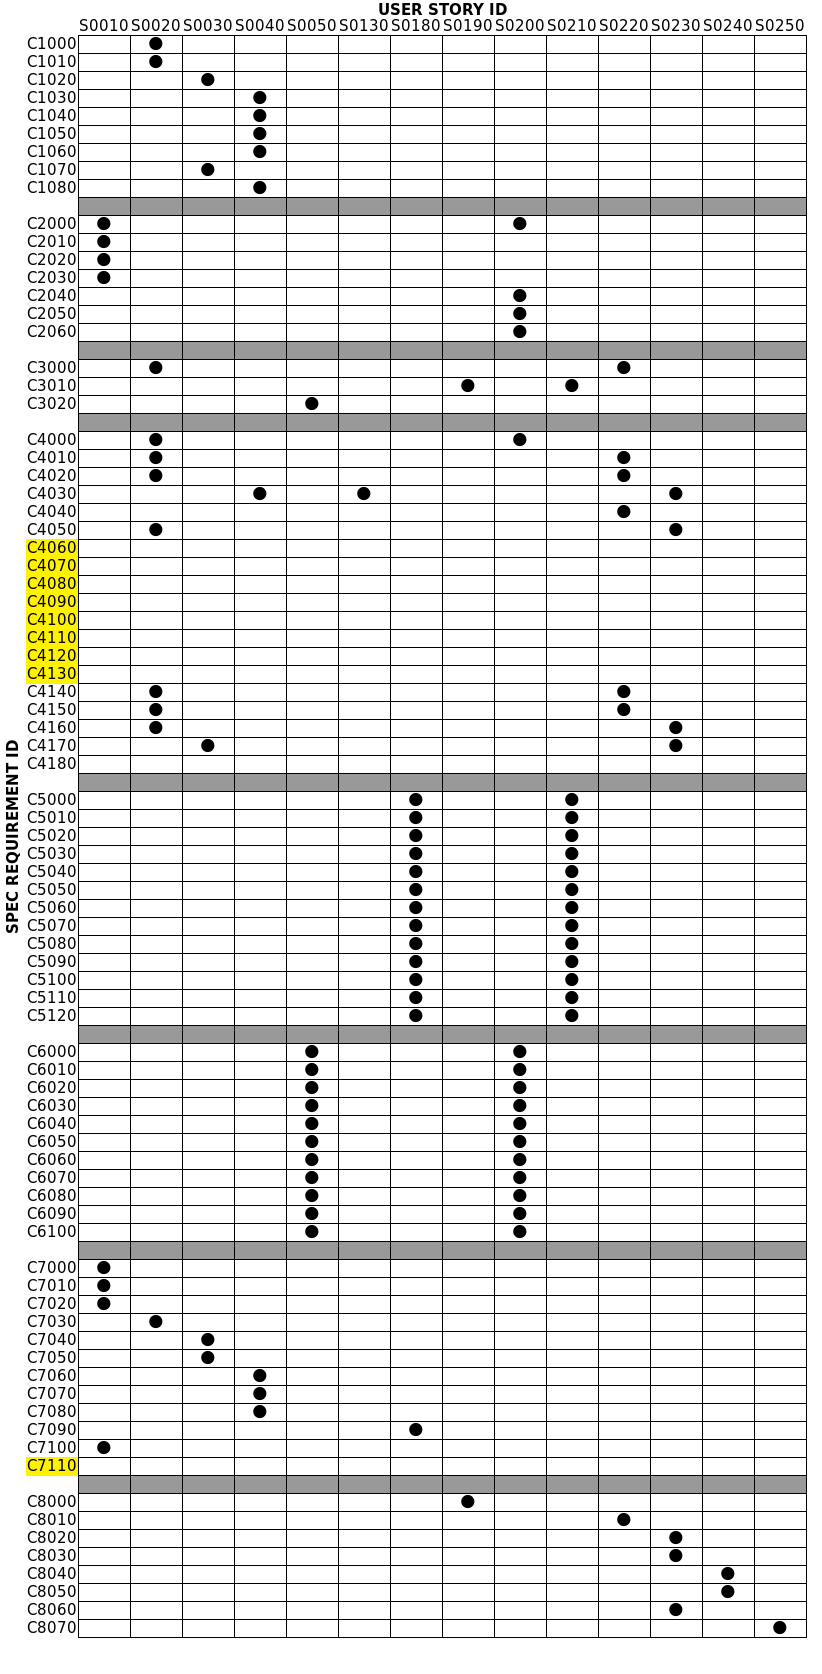
\includepdf[pages=-]{coverage_matrix.pdf}

\end{document}